\documentclass{article}
\usepackage{amsmath}
\usepackage{graphicx}  % Paquete para incluir imágenes
\usepackage{float}
\usepackage{amsmath,amssymb}
\usepackage{geometry}
\geometry{top=2cm, bottom=2cm, left=2.5cm, right=2.5cm}

\begin{document}
Alberto Arath Figueroa Salomon 
\newpage
\begin{flushleft}
Se tiene una neurona con los siguientes pesos $w_0=-4$, $w_1=3$, $w_2=1$ y función de activación
Hacer lo siguiente:

\begin{enumerate}
\item Dibuje la neurona con sus pesos y sus entradas y salida mostrando la entrada que está fija a 1.
\item Calcular el producto $W^T X$ y graficarlo en GeoGebra 3D.
\[ wtx(x_1, x_2) = 3 x_1 + x_2 - 4 \]
\begin{figure}[H]
  \centering
  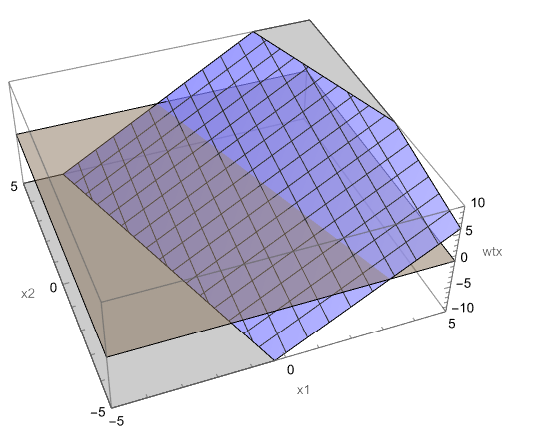
\includegraphics[width=0.5\textwidth]{Imagen0.png}  % Cambia el nombre del archivo y su ruta según sea necesario
\end{figure}
\item Encontrar la ecuación de la recta que divide al espacio de entrada en 2 partes y graficarla usando GeoGebra 2D.
\[ 0 = 3 x_1 + x_2 - 4 \]
\begin{figure}[H]
  \centering
  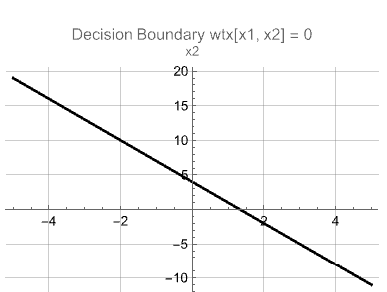
\includegraphics[width=0.5\textwidth]{Imagen1.png}  % Cambia el nombre del archivo y su ruta según sea necesario
\end{figure}
\newpage
\item Graficar en GeoGebra 3D la salida de la neurona $y$.
\begin{figure}[H]
  \centering
  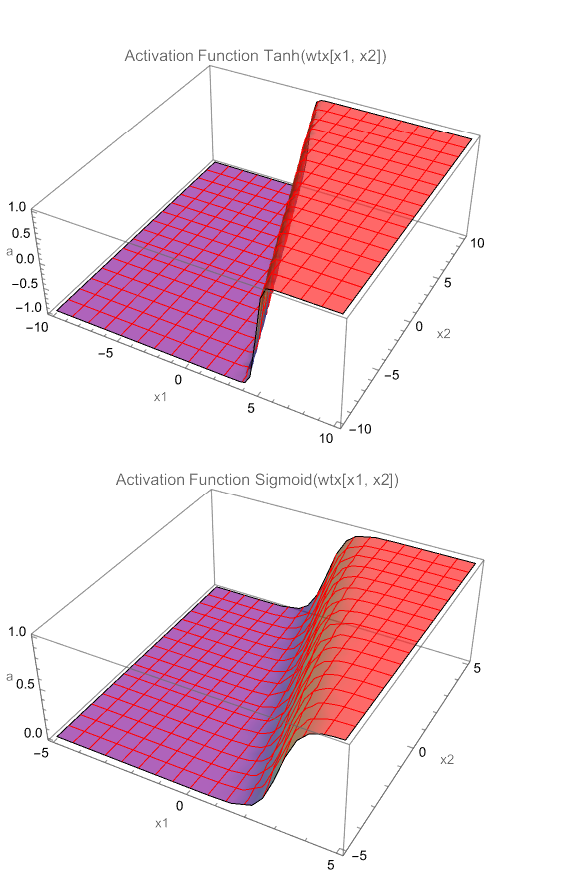
\includegraphics[width=0.5\textwidth]{1d.png}  % Cambia el nombre del archivo y su ruta según sea necesario
\end{figure}
\end{enumerate}
a
\end{flushleft}
\end{document}